%% LyX 2.3.2-2 created this file.  For more info, see http://www.lyx.org/.
%% Do not edit unless you really know what you are doing.
\documentclass[12pt,british,UKenglish]{article}
\renewcommand{\rmdefault}{ptm}
\usepackage[T1]{fontenc}
\usepackage[latin9]{inputenc}
\usepackage[a4paper]{geometry}
\geometry{verbose,tmargin=2cm,bmargin=2cm,lmargin=2.5cm,rmargin=2.5cm}
\setlength{\parskip}{\medskipamount}
\setlength{\parindent}{0pt}
\usepackage{color}
\usepackage{array}
\usepackage{longtable}
\usepackage{booktabs}
\usepackage{calc}
\usepackage{pdfpages}
\usepackage{amsmath}
\usepackage{amssymb}
\usepackage{nomencl}
% the following is useful when we have the old nomencl.sty package
\providecommand{\printnomenclature}{\printglossary}
\providecommand{\makenomenclature}{\makeglossary}
\makenomenclature

\makeatletter

%%%%%%%%%%%%%%%%%%%%%%%%%%%%%% LyX specific LaTeX commands.
%% Because html converters don't know tabularnewline
\providecommand{\tabularnewline}{\\}
%% A simple dot to overcome graphicx limitations
\newcommand{\lyxdot}{.}


%%%%%%%%%%%%%%%%%%%%%%%%%%%%%% Textclass specific LaTeX commands.
\newlength{\lyxlabelwidth}      % auxiliary length 

%%%%%%%%%%%%%%%%%%%%%%%%%%%%%% User specified LaTeX commands.
% -------------------------- Hyperlinks Settings --------------------------
\usepackage{xcolor} % Colours for hyperref package
% Define links colour
\newcommand{\linksColour}{black} 
% hyperref package
\usepackage[colorlinks = true,linkcolor = \linksColour, citecolor = \linksColour, urlcolor = blue ,bookmarksnumbered=true,bookmarksopen = true,bookmarksopenlevel = 1]{hyperref}
% ------------------------------------------------------------------------------

% -------------------- Header and Footer Settings --------------------
% Header and footer
\usepackage{fancyhdr}
\pagestyle{fancy}
\fancyhead{} 	             % clear the default header
\fancyfoot{}                % clear the default footer
\fancyfoot[C]{\footnotesize\thepage}     % page number in the middle
\renewcommand{\headrulewidth}{0.0pt}  % remove the default header line

% Header and footer of automatically generated pages (e.g. TOC)
% Change to match main document
\fancypagestyle{plain}{
\fancyhead{}
\fancyfoot{}
\fancyfoot[C]{\footnotesize\thepage}
\renewcommand{\headrulewidth}{0pt}}

% ------------------------------------------------------------------------------

% ------------------------ Title Page Box Settings -------------------------
% settings for the text box on the front page
\newcommand\HRule{\noindent\rule{\linewidth}{2pt}}
% ------------------------------------------------------------------------------


% -------------------------- Figures Settings -----------------------------
% Redefine how latex deals with figure placement
\renewcommand{\topfraction}{.85}
\renewcommand{\bottomfraction}{.7}
\renewcommand{\textfraction}{.15}
\renewcommand{\floatpagefraction}{.66}
\renewcommand{\dbltopfraction}{.66}
\renewcommand{\dblfloatpagefraction}{.66}
% ------------------------------------------------------------------------------


% ------------------------------ TOC Settings --------------------------------

% Adding dots to sections in table of contents
\usepackage{tocloft}
\renewcommand{\cftloftitlefont}{\large\bfseries}
\renewcommand{\cftlottitlefont}{\large\bfseries}
\renewcommand{\cftsecleader}{\cftdotfill{\cftdotsep}}
% Adding the word Figure in list of figures
\renewcommand*\cftfigpresnum{Figure~}
\settowidth{\cftfignumwidth}{\cftfigpresnum}
\renewcommand{\cftfigaftersnumb}{\qquad}
% Adding the word Table in list of figures
\renewcommand*\cfttabpresnum{Table~}
\settowidth{\cfttabnumwidth}{\cfttabpresnum}
\renewcommand{\cfttabaftersnumb}{\qquad}
% ------------------------------------------------------------------------------

% Changing the rules for hyphenation (DON"T CHANGE THIS)
\usepackage{everysel}
\EverySelectfont{%
\fontdimen2\font=0.4em% interword space
\fontdimen3\font=0.2em% interword stretch
\fontdimen4\font=0.1em% interword shrink
\fontdimen7\font=0.1em% extra space
\hyphenchar\font=`\-% to allow hyphenation
}

% -------------------- Formatting Section Titles ------------------------
% Shrinking the space after headers
\usepackage[clearempty]{titlesec} % loaded with a setting for automatically generated empty pages to be completely blank
\beforetitleunit = 1pt
\aftertitleunit = 1pt
% specifying the spacing before and after the titles (note \parskip = 9pts)
\titlespacing{\section}{0pt}{*9}{*9}	% for 18 pt space
\titlespacing{\subsection}{0pt}{*3}{*3}	% for 12 pt space
\titlespacing{\subsubsection}{0pt}{*3}{*3}	% for 12 pt space
% specifying the title fomatting
\titleformat{\section} {\normalfont\fontsize{14}{14}\bfseries}{\thesection.}{1em}{}
\titleformat{\subsection} {\normalfont\fontsize{12}{12}\bfseries}{\thesubsection}{1em}{}
\titleformat{\subsubsection} {\normalfont\fontsize{12}{12}\it}{\thesubsubsection}{1em}{}

% Modifyong how appendices look (title and toc)
\usepackage[titletoc,title]{appendix}
% ------------------------------------------------------------------------------

% ------------------------- Nomenclature Settings ------------------------

\def\nompreamble{\addcontentsline{toc}{section}{\nomname}\markboth{\nomname}{\nomname}}
% cutomising nomenclature groups
\usepackage{ifthen}
\renewcommand{\nomgroup}[1]{ 
\ifthenelse{\equal{#1}{A}}{\item[\textbf{Symbols}]}{%
\ifthenelse{\equal{#1}{G}}{\item[\textbf{Greek Symbols}]}{}
}% matches Greek Symbols
}% matches Roman Symbols

% unit column in nomenclature
\newcommand{\nomunit}[1]{\renewcommand{\nomentryend}{\hspace*{\fill}#1}}

% ------------------------------------------------------------------------------

% -------------------------- Miscellaneous Settings ----------------------------

% disable automatic date printing (otherwise will mess with the title page)
\date{} 
\usepackage{babel}% http://ctan.org/pkg/babel
\usepackage{isodate}% http://ctan.org/pkg/isodate

% Group sequential citations (cite is incompatible with biblatex, so skip it when biblatex is loaded)
\csname @ifpackageloaded\endcsname{biblatex}{}{\usepackage{cite}}

%\usepackage{keystroke} % Keyboard symbols 
\usepackage{breakurl}    % break long urls (not sure if it works by default)
\urlstyle{rm}	                  % Change url fonts to match report font

% to allow page breaks within equations
\allowdisplaybreaks

% force footnotes to be always at the bottom of the page
\usepackage[bottom]{footmisc} 

% For tables with merged rows
\usepackage{multirow}

\usepackage[labelfont={bf,footnotesize},textfont={footnotesize}, labelsep = quad]{caption}

\usepackage{units}

% load listings package for code envirnments
\usepackage{listings}
% ------------------------------------------------------------------------------

\usepackage{menukeys} % for menu instructions % import additional settings from this file

\makeatother

\usepackage{babel}
\usepackage{listings}
\lstset{basicstyle={\ttfamily\footnotesize},
belowcaptionskip=3mm,
breaklines=true,
commentstyle={\color[rgb]{0,0.5,0}},
frameshape={{NYN}{nnn}{nnn}{NYN}},
keywordstyle={\color{blue}},
language=Matlab,
numbers=left,
numberstyle={\scriptsize},
showstringspaces=false,
stringstyle={\color{purple}}}
\def\eqdeclaration#1{, see equation\nobreakspace(#1)}
\def\pagedeclaration#1{, page\nobreakspace#1}
\def\nomname{Nomenclature}
\renewcommand{\lstlistingname}{Listing}

\begin{document}
% Define your name and report number here. It will update on all pages where they are needed.
\def \name{[Add Your Name]}
\def \reportNumber{ME000-\the\year}

%% -------------------------------------------------------------------------------------------
%% ---------------------------- Title page of the report -------------------------------------
%% -------------------------------------------------------------------------------------------
\thispagestyle{empty}
\pagenumbering{roman}
% Change default name for code environments
\renewcommand\lstlistingname{Program}  

\vspace*{10mm}

\begin{center}
\textbf{\large{}Research Project in Mechanical <or Mechatronics> Engineering}{\large\par} % UPDATE this to match your specialisation
\par\end{center}

\vspace*{10mm}

\HRule
\begin{center}
Type of Report
\par\end{center}

\begin{center}
\textbf{\Large{}Project Title Goes Here}{\Large\par}
\par\end{center}

\begin{center}
{\large{}\name}{\large\par}
\par\end{center}

\begin{center}
Project Report \reportNumber
\par\end{center}

\HRule

\vspace*{\fill}

\begin{center}
\begin{tabular}{rl}
Co-worker: & {[}Add Partner{]}\tabularnewline   % ADD your partner's name here
\noalign{\vskip1.5em}
Supervisor: & Dr {[}Add Supervisor{]}\tabularnewline    % ADD your supervisor's name here
\noalign{\vskip1.5em}
\end{tabular}
\par\end{center}

\vspace*{\fill}

\begin{center}
\cleanlookdateon \today
\par\end{center}

\vspace*{\fill}

\begin{center}

\includegraphics[width=0.7\linewidth]{Figures/mech-horizontal-hc}
\par\end{center}

\newpage{}
%% -------------------------------------------------------------------------------------------
%% ---------------------------- Frontmatter of the report ------------------------------------
%% -------------------------------------------------------------------------------------------

%% ----------------------------------- ABSTRACT ----------------------------------------------
\begin{flushleft}
\reportNumber
\par\end{flushleft}

\vspace{1em}

\begin{center}
\textbf{\textsc{\large{}PROJECT TITLE GOES HERE}}{\large\par}
\par\end{center}

\vspace{2em}

\begin{center}
\textbf{\large{}\name}{\large\par}
\par\end{center}

\vspace{2em}

\begin{center}
\textbf{\textsc{\large{}ABSTRACT}}{\large\par}
\par\end{center}
% Write your abstract here
Abstract goes here.
% end of Abstract

%% ------------------------------- DECLARATION -------------------------------------------
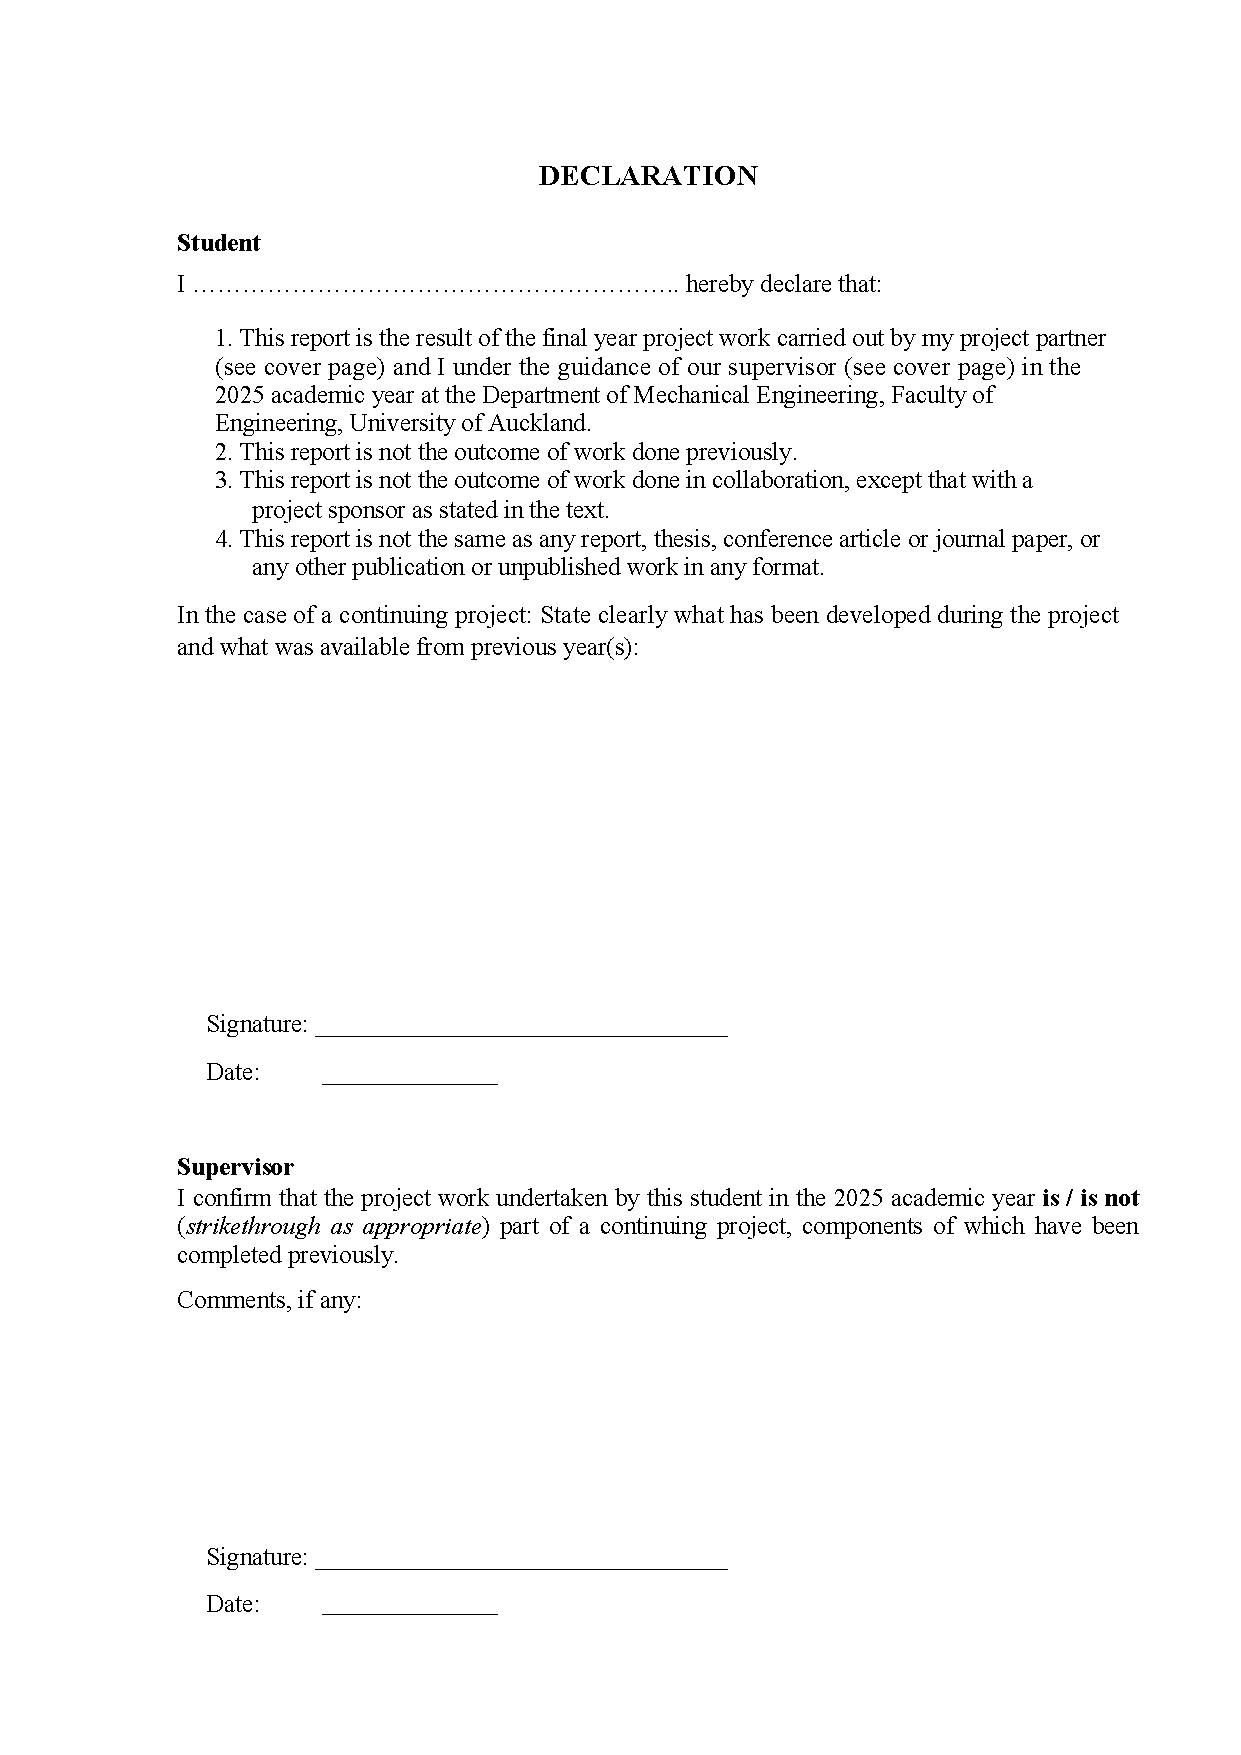
\includepdf[pagecommand=\thispagestyle{fancy}]{Declaration} % Overwrite the PDF in the root folder to update with the signed document.
    

\newpage{}
%% ------------------------------ TABLE OF CONTENTS ---------------------------------------
\setlength{\parskip}{6pt}
\renewcommand{\contentsname}{\large{Table of Contents}}

\tableofcontents{}

\newpage{}

\setlength{\parskip}{9pt}
%% ------------------------------- ACKNOWLEDGMENTS -------------------------------------------
\section*{Acknowledgements \addcontentsline{toc}{section}{Acknowledgements}\label{sec:Acknowledgements1}}

Thank important people here.

\newpage{}
%% ------------------------------- GLOSSARY -------------------------------------------
\section*{Glossary of Terms \addcontentsline{toc}{section}{Glossary of Terms}}

\begin{longtable}[l]{>{\raggedright}p{0.25\textwidth}>{\raggedright}p{0.7\textwidth}}
Term & Definition\tabularnewline
\addlinespace
\end{longtable}

\addtocounter{table}{-1}
%% ------------------------------- ABBREVIATIONS -------------------------------------------
\section*{Abbreviations\addcontentsline{toc}{section}{Abbreviations}}

\begin{longtable}[l]{>{\raggedright}p{0.25\textwidth}>{\raggedright}p{0.7\textwidth}}
AOA & Angle of attack\tabularnewline
\addlinespace
\end{longtable}

\addtocounter{table}{-1}
%% ------------------------------- NOMENCLATURE -------------------------------------------
\printnomenclature{}\label{nomenclature}

\clearpage{}

\setlength{\parskip}{9pt}

\pagenumbering{arabic}

%% -------------------------------------------------------------------------------------------
%% ---------------------------- Main Body of the report --------------------------------------
%% -------------------------------------------------------------------------------------------

\section{Introduction}

Some text \cite{Balas1998}.

\subsection{Subsection}

Some text.


%% ------------------------------- REFERENCES -------------------------------------------
\bibliographystyle{IEEEtran}
\addcontentsline{toc}{section}{\refname}\bibliography{RefDatabase}

\newpage{}

%% -------------------------------------------------------------------------------------------
%% ----------------------------------- APPENDICES---------------------------------------------
%% -------------------------------------------------------------------------------------------
\begin{appendices}
\titleformat{\section} {\normalfont\fontsize{14}{14}\bfseries}{Appendix~\thesection}{1em}{}

% Renaming the captions to include the appendix name
\renewcommand{\theequation}{\thesection \arabic{equation}}
\renewcommand{\thefigure}{\thesection \arabic{figure}}
\renewcommand{\thetable}{\thesection \arabic{table}}
\renewcommand{\thelstlisting}{\thesection \arabic{lstlisting}}

\section{The First Appendix}

\setcounter{equation}{0}
\setcounter{figure}{0}
\setcounter{table}{0}
\setcounter{lstlisting}{0}

\begin{lstlisting}[caption={Some MATLAB script},label={lis:Same-MATLAB-script}]
% SaveExperiment.m: This file prompts the user to save the data
% and plots the results.
% 
% This file is meant to be run autoamtically after lab experiment is
% finished. 
% 
% Hazim Namik                           Date created: 14/4/2019

clc;

% prompting the user to specify a file name and a location
[fileName,filePath] = uiputfile('*.mat','Save file name');
% Checking if the user clicked cancel
if(~(ischar(fileName)&& ischar(filePath)))
    disp('Canceled. No data was saved.');
    return
end
% Saving the file at the specified location
save ([filePath,fileName],'ActualPumpUsage', 'ActualError', 'TankHeightAll', 'SimPumpUsage', 'SimError');
\end{lstlisting}

\clearpage{}

\section{Second Appendix}

\setcounter{equation}{0}
\setcounter{figure}{0}
\setcounter{table}{0}
\setcounter{lstlisting}{0}

\end{appendices}
% -------------------------- End of Appendices --------------------------------

\end{document}
%% -----------------------------  END OF DOCUMENT --------------------------------